\chapter{Research Design and Strategies}
\label{chapter:4}

Given the non-existence of standards for federated social networks, we define
the following research questions to guide this work.

\begin{description}
  \item [\textit{RQ1:}]
    \textit{What are the protocols in use for federation of social networks and
    what is the status of their development and adoption?}
    During the development of this research, we explored the protocols proposed
    and being used to approach the implementation of federated social networks,
    reporting the current status of the alternatives and projects that use it.

  \item [\textit{RQ2:}]
    \textit{What engineering problems need to be solved in order to add support for
    federation in a platform that was not conceived with federation as a
    requirement?}
    There is virtually no literature on the implementation of federation support on
    existent projects. Most of the previous work describe the design and
    implementation of federated systems, without assuming a previous, non-federated
    system. We wanted to investigate which aspects of a project can affect the
    implementation of federation support.
\end{description}

\section{Design Alternatives}

There are currently two possible strategies for implementing federation. Some
of the discussion on this topic is recorded in W3C mailing lists\footnote{In
the following thread from the federated social networks group
\url{http://lists.w3.org/Archives/Public/public-fedsocweb/2013May/0058.html}}
and we have organized them to be presented in this section.

We could have the development of a system or protocol that should
be supported by all applications interested in joining the federation, a
method characterized by a sole entity acting as the common denominator
among all networks, or alternatively by a massive coordination effort
among loosely-coupled, independent projects working on the topic.

The alternative is every application explicitly implementing the
protocol of every other application it wants to connect with. This
strategy does not depend on a standard protocol, or on a central
authority to define what needs to be implemented and how. It can be
called the ``polyglot strategy''.

The polyglot strategy brings some restrictions to the federation of
systems, since it depends on every application responding to the
protocol of every other application in the network. This strategy seems
to support the segmentation of specifications as opposed to what would
happen when using a single protocol as the common denominator.  On the
other hand, the adoption of a common denominator depends on a protocol
capable of covering the peculiarities of all possible networks, including
types of relationships among users, content sharing mechanisms, and
privacy policies.

The criticism over the lack of a notion of privacy in
OStatus\footnote{The discussion regarding OStatus privacy can also be
found in W3C mailing lists,
\url{http://lists.w3.org/Archives/Public/public-fedsocweb/2013May/0061.html}.}
is an example of the barriers caused by these differences. The project
only supports public content, so networks with more complex privacy
definitions are not completely covered. In the meantime, other projects were
created to cover these flaws, such as Diaspora and Friendica.

A specification that meets the requirements of all possible social
networks would require a very large design and development effort. An
alternative would be a protocol that establishes a subset of policies as
a base to the implementation of more complex or specific features. It
can be argued that, eventually, these policies would have to support
incompatible concepts, given the difficulty of finding ways to satisfy
all systems.

\begin{figure}[!hbt]
  \centering
  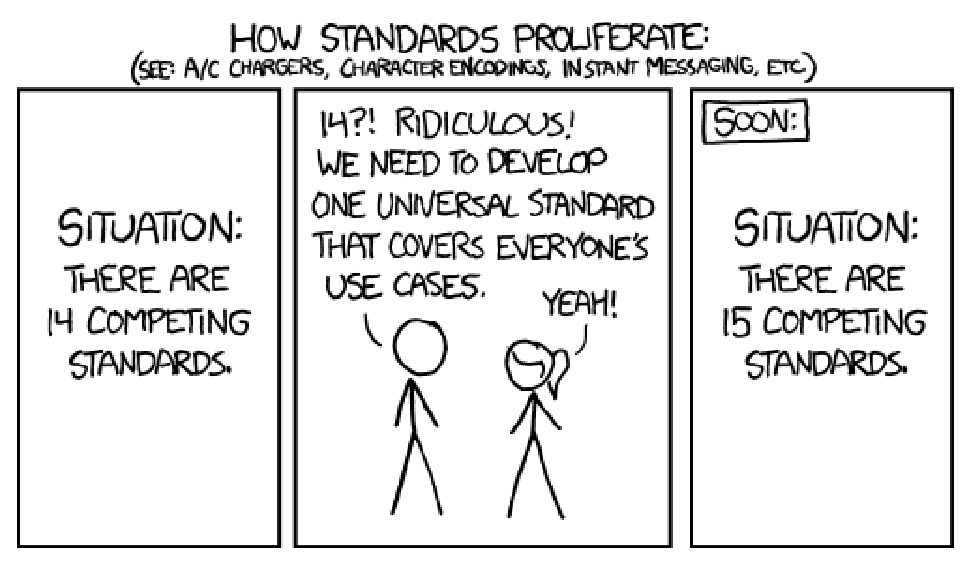
\includegraphics[width=0.45\textwidth]{figures/xkcd-standards.eps}
  \caption{XKCD: Standards. Source: \url{https://xkcd.com/927}}
  \label{fig:xkcd_standards}
\end{figure}

Even if such an agreement could be found, every application would have to solve
its own needs based on the restrictions of the common denominator. It would
possibly require projects to be heavily modified to adopt such a protocol,
which does not contribute to the viability of that strategy.

The tendency to adopt a polyglot strategy indicates that the difficulty
in finding a universal common denominator surpasses the interoperability
benefits. On the other hand, if projects keep implementing integration
with individual projects we could eventually find some kind of
convergence, leading to a network effect, and identifying a common
denominator for a subset of applications.

For now, federation can only be achieved by a polyglot strategy, adopting
the specifications of individual projects, which are usually a suite of
well established protocols. A good start is to choose a project
considering its community activity and the adherence of its standard
with your particular needs.

\section{Case study: Noosfero}

Noosfero\footnote{\url{http://noosfero.org}} is our free software
platform that can be used to build social and collaboration networks,
providing a platform with blogs, CMS, and feeds. It is written in Ruby,
using the Rails framework, is licensed under the Affero GNU General
Public License version 3, and has an active development community.

The need for supporting federation is a long-standing issue for the
Noosfero project. Started in 2007, when the ideas around federation were
still incipient, Noosfero ended up evolving a large set of features
required by the different organizations that use it before a proper
plan for adding federation could be laid out.

We decided to spearhead the development of federation support in
Noosfero, with the main goal of allowing Noosfero sites to integrate with
other social network providers, whether they also use Noosfero, or
not. Our proposal was to use the Diaspora protocol.

Even though the objective is to eventually support the entire protocol,
the first step was producing a proof of concept that implements a subset
of it. This would help identifying the required modifications in the
Noosfero code, and designing the rest of the federation infrastructure.
It will provide an initial level of federation that can already be
used by end users.

To define the scope of this proof of concept we took into consideration
roadmaps that were result of previous discussions in the community. We derived
the following requirements from the features we believe will help the most to
build the federation infrastructure, mainly the users discovery and message
exchange mechanisms.

\begin{enumerate}
  \item
    Remote users must be located via the Noosfero people search. The
    implementation must follow the discovery standard used by
    Diaspora, based on WebFinger. It must also be possible to find
    Noosfero users from any other Noosfero or Diaspora site.

  \item
    Users from a Noosfero and a Diaspora site must be able to follow
    each other. Both sides must be aware of the relationship.

  \item
    The Noosfero server should receive and handle publications sent by
    Diaspora servers, making it possible to consume contents from remote
    servers. Sending these messages from Noosfero will make it possible
    for local users to be followed, what is also the scope of the proof
    of concept.

  \item
    Noosfero sites should also send publications and comments to any
    other server that hosts a user that follows the activity of local profiles.
    This adds symmetry to the previous feature, providing reciprocal interaction
    between the servers.
\end{enumerate}
